%%%%%%%%%%%%%%%%%%%%%%%%
%
% $Autor: Hemanth Jadiswami Prabhakaran $
% $Datum: 2025-06-29 19:46:27Z $
% $Pfad: GitHub/BA25-01-Time-Series/report/Contents/en/matplotlib.tex $
% $Version: 1 $
%
% $Project: BA25-Time-Series $
%
%%%%%%%%%%%%%%%%%%%%%%%%


%
% !TeX encoding = utf8
% !TeX root = PythonPackages
%
%%%%%%%%%%%%%%%%%%%%%%%%

\chapter{Matplotlib}
\label{ch:matplotlib}

\section{Introduction}
\label{sec:matplotlib_intro}

Matplotlib stands as the foundational visualization library for Python, serving as the cornerstone of scientific plotting and data visualization since its inception in 2003 by John D. Hunter \cite{Hunter:2007}. Drawing inspiration from MATLAB's plotting capabilities, Matplotlib has evolved into a comprehensive 2D plotting library that provides publication-quality figures across a wide range of hardcopy formats and interactive environments \cite{Matplotlib:2024}. The library's significance extends beyond simple plotting, as it serves as the backend for numerous higher-level visualization libraries including seaborn, pandas plotting, and scikit-learn's visualization utilities. This chapter provides comprehensive coverage of Matplotlib's capabilities, from basic plotting to advanced customization techniques, enabling readers to create professional-grade visualizations for scientific, engineering, and business applications.\\

The importance of Matplotlib in the Python ecosystem cannot be overstated, as it bridges the gap between data analysis and visual communication \cite{VanderPlas:2016}. Modern data science workflows rely heavily on effective visualization for exploratory data analysis, model validation, and result presentation. Matplotlib's object-oriented architecture and extensive customization options make it suitable for both quick exploratory plots and publication-ready figures \cite{Droettboom:2021}. The library's integration with NumPy arrays and compatibility with interactive environments like Jupyter notebooks has established it as an essential tool for scientists, engineers, and data analysts worldwide. Understanding Matplotlib's architecture and capabilities is crucial for anyone working with data visualization in Python.\\

\section{Description}
\label{sec:matplotlib_description}

\subsection{Core Capabilities}
\label{subsec:matplotlib_capabilities}

Matplotlib offers a comprehensive suite of visualization capabilities:

\begin{itemize}
	\item \textbf{2D Plotting}: Line plots, scatter plots, bar charts, histograms, and heatmaps
	\item \textbf{Statistical Visualization}: Box plots, violin plots, error bars, and regression plots
	\item \textbf{Scientific Plotting}: Contour plots, vector fields, polar plots, and 3D visualizations
	\item \textbf{Customization}: Complete control over colors, fonts, styles, and layout
	\item \textbf{Export Formats}: Vector and raster formats including PDF, SVG, PNG, and EPS
\end{itemize}

\clearpage

\subsection{Python Framework: matplotlib}
\label{subsec:matplotlib}

The \texttt{matplotlib} package provides both MATLAB-style (pyplot) and object-oriented interfaces for creating visualizations:

\begin{lstlisting}[language=MyPython, caption={Matplotlib Core Functions}, label={lst:matplotlib_core}]
	
	import matplotlib.pyplot as plt
	import numpy as np
	
	# MATLAB-style interface
	x = np.linspace(0, 10, 100)
	y = np.sin(x)
	plt.plot(x, y)
	plt.xlabel('X values')
	plt.ylabel('Y values')
	plt.title('Sine Function')
	plt.show()
	
	# Object-oriented interface
	fig, ax = plt.subplots()
	ax.plot(x, y)
	ax.set_xlabel('X values')
	ax.set_ylabel('Y values')
	ax.set_title('Sine Function')
	plt.show()
	
\end{lstlisting}

\subsection{Use Cases}
\label{subsec:matplotlib_usecases}

Matplotlib finds applications across diverse domains:

\begin{enumerate}
	\item \textbf{Scientific Research}: Publication-quality plots for research papers and presentations
	\item \textbf{Data Analysis}: Exploratory data analysis and statistical visualization
	\item \textbf{Engineering}: Technical plots for system analysis and simulation results
	\item \textbf{Business Intelligence}: Dashboard creation and report generation
	\item \textbf{Education}: Teaching aids and interactive learning materials
\end{enumerate}

\subsection{Architecture Overview}
\label{subsec:matplotlib_architecture}

\begin{figure}[H]
	\centering
	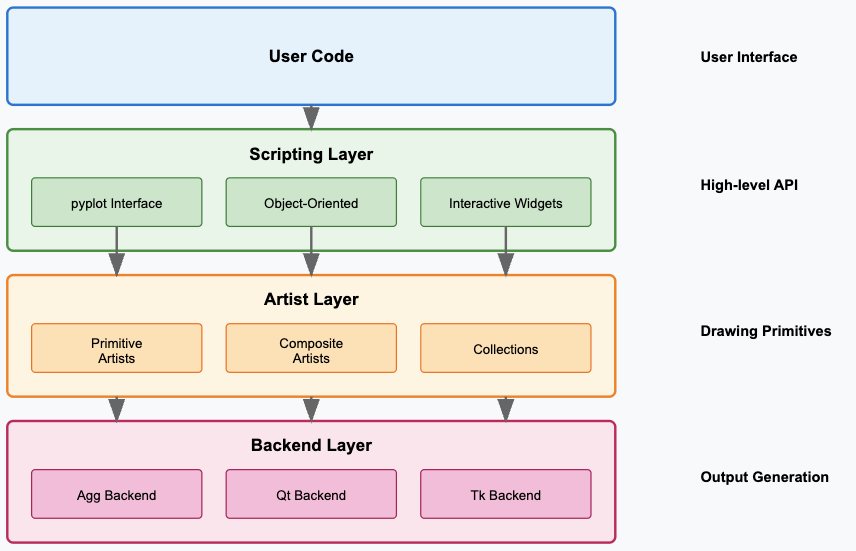
\includegraphics[width=1\textwidth]{Images/matplotlib/matplotlibArchitecture.png}
	\caption{Matplotlib Architecture Components \cite{Matplotlib:2024}}
	\label{fig:matplotlib_architecture}
\end{figure}

The Matplotlib architecture consists of three main layers, as illustrated in Figure \ref{fig:matplotlib_architecture}. The Backend layer handles rendering to different output formats, the Artist layer manages drawing primitives, and the Scripting layer provides user-friendly interfaces \cite{Hunter:2007}. This layered architecture enables both simple plotting and fine-grained control over every aspect of the visualization.

\clearpage

\section{Installation}
\label{sec:matplotlib_installation}

\subsection{System Requirements}
\label{subsec:matplotlib_system_requirements}

Matplotlib requires Python 3.8 or higher and has several optional dependencies for enhanced functionality. The library works across all major operating systems with minimal system-specific requirements.

\subsection{Python Package Installation}
\label{subsec:matplotlib_python_install}

Install Matplotlib using pip:

\begin{lstlisting}[style=bashstyle, caption={Matplotlib Installation}]
	# Basic installation
	pip install matplotlib
	
	# Installation with common scientific libraries
	pip install matplotlib numpy pandas scipy
	
	# For development and testing
	pip install matplotlib[dev]
	
	# With additional backends
	pip install matplotlib[gui]
\end{lstlisting}

\subsection{Backend Configuration}
\label{subsec:backend_config}

Matplotlib supports multiple backends for different output formats and interactive environments:

\begin{lstlisting}[language=MyPython, caption={Backend Configuration}, label={lst:backend_config}]
	import matplotlib
	
	# List available backends
	print(matplotlib.backend_bases.Backend.list())
	
	# Set backend programmatically
	matplotlib.use('Agg')  # Non-interactive backend
	
	# Check current backend
	print(matplotlib.get_backend())
\end{lstlisting}

\subsection{Verification}
\label{subsec:matplotlib_verification}

Verify the installation by creating a simple plot:

\begin{lstlisting}[language=MyPython, caption={Installation Verification}, label={lst:verification}]
	import matplotlib.pyplot as plt
	import numpy as np
	
	x = np.linspace(0, 2*np.pi, 100)
	y = np.sin(x)
	plt.plot(x, y)
	plt.title('Matplotlib Installation Test')
	plt.show()
\end{lstlisting}

\section{Example -- Basic Plotting}
\label{sec:matplotlib_basic_example}

The following example demonstrates fundamental plotting capabilities including line plots, scatter plots, and basic customization. The complete implementation is available in \texttt{BasicPlotting.py}.

\lstinputlisting[language=MyPython, caption={Basic Matplotlib Plotting}, label={lst:matplotlib_basicplotting}]{../Code/matplotlib/BasicPlotting.py}

This basic example illustrates the core Matplotlib workflow: data preparation, plot creation, customization, and display. The example showcases both the pyplot interface and basic styling options that form the foundation of effective data visualization.

\section{Example -- Advanced Visualization}
\label{sec:advanced_example}

Advanced Matplotlib applications leverage subplots, statistical plots, and sophisticated styling for comprehensive data analysis. The integration of multiple plot types enables complex visual narratives.

\clearpage

\begin{figure}[htbp]
	\centering
    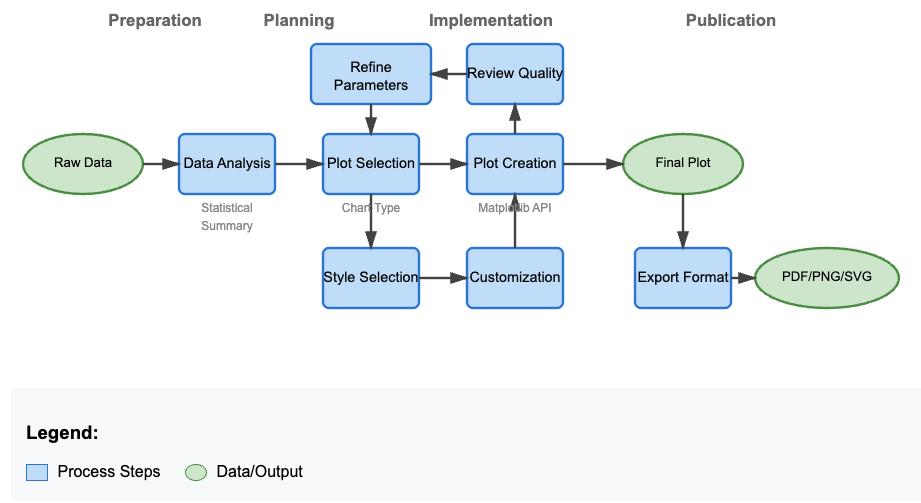
\includegraphics[width=1\textwidth]{Images/matplotlib//visualizationWorkflow.png}
	\caption{Advanced Visualization Workflow}
	\label{fig:visualization_workflow}
\end{figure}

The visualization workflow illustrated in Figure \ref{fig:visualization_workflow} shows the process from data input through analysis to final presentation-ready plots.

\lstinputlisting[language=MyPython, caption={Advanced Matplotlib Visualization}, label={lst:matplotlib_advancedvisualization}]{../Code/matplotlib/AdvancedVisualization.py}

\section{Example -- Scientific Plotting}
\label{sec:scientific_example}

Scientific applications require specialized plot types including contour plots, 3D visualizations, and mathematical function plotting. Matplotlib provides comprehensive support for technical and scientific visualization needs.

\begin{figure}[htbp]
	\centering
    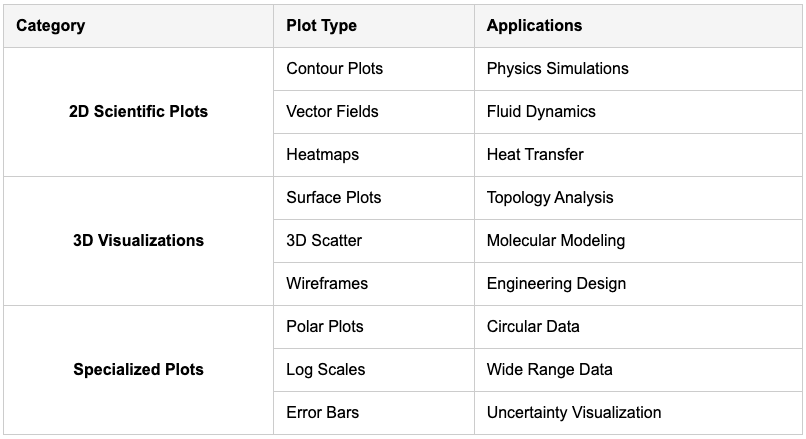
\includegraphics[width=1\textwidth]{Images/matplotlib/scientificPlotting.png}
	\caption{Scientific Plotting Capabilities}
	\label{fig:scientific_plotting}
\end{figure}

The scientific plotting capabilities illustrated in Figure \ref{fig:scientific_plotting} demonstrate the range of specialized visualizations available for research and engineering applications.

\lstinputlisting[language=MyPython, caption={Scientific Plotting with Matplotlib}, label={lst:matplotlib_scientificplotting},firstline=1,lastline=50]{../Code/matplotlib/ScientificPlotting.py}

\noindent\textit{[The remaining code is omitted for brevity. The complete script can be found at \texttt{../Code/matplotlib/ScientificPlotting.py}.]}

\section{Example -- Interactive and Animated Plots}
\label{sec:interactive_example}

Interactive and animated visualizations enhance user engagement and enable dynamic data exploration. Matplotlib supports both widget-based interactivity and time-based animations.

\lstinputlisting[language=MyPython, caption={Interactive and Animated Plots}, label={lst:matplotlib_interactiveplots},firstline=1,lastline=50]{../Code/matplotlib/InteractivePlots.py}

\noindent\textit{[The remaining code is omitted for brevity. The complete script can be found at \texttt{../Code/matplotlib/InteractivePlots.py}.]}

\section{Performance Optimization}
\label{sec:matplotlib_optimization}

Optimizing Matplotlib performance requires understanding rendering backends, memory management, and efficient plotting techniques. Proper optimization ensures responsive visualization even with large datasets.

\subsection{Backend Selection}
\label{subsec:backend_selection}

Choosing appropriate backends for different use cases:

\begin{lstlisting}[language=MyPython, caption={Backend Optimization}, label={lst:backend_optimization}]
	import matplotlib
	
	# Non-interactive backend for batch processing
	matplotlib.use('Agg')
	
	# Interactive backends for exploration
	# matplotlib.use('Qt5Agg')  # For Qt applications
	# matplotlib.use('TkAgg')   # For Tkinter applications
	
	# Vector backends for publication
	# matplotlib.use('PDF')     # For PDF output
	# matplotlib.use('SVG')     # For SVG output
\end{lstlisting}

\subsection{Large Dataset Handling}
\label{subsec:large_datasets}

Techniques for handling large datasets efficiently:

\begin{lstlisting}[language=MyPython, caption={Large Dataset Optimization}, label={lst:large_datasets}]
	import matplotlib.pyplot as plt
	import numpy as np
	
	# Data aggregation for large datasets
	def downsample_data(x, y, max_points=1000):
	    if len(x) <= max_points:
	        return x, y
	    
	    indices = np.linspace(0, len(x)-1, max_points, dtype=int)
	    return x[indices], y[indices]
	
	# Efficient plotting with rasterization
	fig, ax = plt.subplots()
	ax.plot(x, y, rasterized=True)  # Rasterize for performance
	ax.set_rasterization_zorder(0)  # Rasterize below this z-order
\end{lstlisting}

\subsection{Memory Management}
\label{subsec:memory_management}

Managing memory usage in visualization applications:

\begin{lstlisting}[language=MyPython, caption={Memory Management}, label={lst:memory_management}]
	import matplotlib.pyplot as plt
	import gc
	
	# Explicit figure cleanup
	fig, ax = plt.subplots()
	# ... plotting code ...
	plt.close(fig)  # Explicitly close figure
	
	# Garbage collection for large visualization loops
	for i in range(1000):
	    fig, ax = plt.subplots()
	    # ... plotting code ...
	    plt.close(fig)
	    
	    if i % 100 == 0:
	        gc.collect()  # Force garbage collection
\end{lstlisting}

\section{Error Handling and Best Practices}
\label{sec:best_practices}

Robust Matplotlib applications must handle various error conditions including data validation, backend issues, and rendering problems. Implementing proper error handling ensures reliable visualization generation.

\subsection{Common Issues and Solutions}
\label{subsec:common_issues}

\begin{enumerate}
	\item \textbf{Backend Issues}: Properly configure backends for different environments
	\item \textbf{Memory Leaks}: Explicitly close figures and manage resources
	\item \textbf{Rendering Problems}: Handle missing fonts and display issues
	\item \textbf{Data Validation}: Validate input data before plotting
\end{enumerate}

\subsection{Error Handling Patterns}
\label{subsec:matplotlib_error_patterns}

\lstinputlisting[language=MyPython, caption={Comprehensive Error Handling with Matplotlib}, label={lst:matplotlib_errorhandling},firstline=1,lastline=50]{../Code/matplotlib/ErrorHandling.py}

\noindent\textit{[The remaining code is omitted for brevity. The complete script can be found at \texttt{../Code/matplotlib/ErrorHandling.py}.]}

\section{Further Reading}
\label{sec:matplotlib_further_reading}

To deepen understanding of Matplotlib and advanced visualization techniques, consider these resources:

\subsection{Official Documentation}
\begin{itemize}
	\item \textbf{Matplotlib Documentation}: \url{https://matplotlib.org/stable/}
	\item \textbf{Matplotlib Gallery}: \url{https://matplotlib.org/stable/gallery/}
	\item \textbf{Matplotlib GitHub Repository}: Official source code repository \cite{Matplotlib:2024}
	\item \textbf{Matplotlib Tutorials}: \url{https://matplotlib.org/stable/tutorials/}
	\item \textbf{Matplotlib Users Guide}: \url{https://matplotlib.org/stable/users/}
\end{itemize}

\subsection{Advanced Topics and Extensions}
\begin{itemize}
	\item \href{https://seaborn.pydata.org/}{Seaborn: Statistical Visualization}
	\item \href{https://plotly.com/python/}{Plotly: Interactive Visualizations}
	\item \href{https://bokeh.org/}{Bokeh: Web-based Visualization}
	\item \href{https://matplotlib.org/basemap/}{Basemap: Geographic Plotting} \cite{VanderPlas:2016}
\end{itemize}

\section{Conclusion}
\label{sec:matplotlib_conclusion}

Matplotlib provides a comprehensive and flexible foundation for data visualization in Python, offering both simplicity for basic plots and sophisticated control for advanced applications. From simple line plots to complex scientific visualizations, Matplotlib's layered architecture and extensive customization options make it indispensable for data analysis, scientific research, and presentation graphics. The examples and techniques presented in this chapter provide a solid foundation for creating effective visualizations, while the architectural understanding enables optimization for specific use cases and performance requirements.\\

Future developments in Matplotlib focus on improved performance, enhanced interactivity, and better integration with modern web technologies \cite{Droettboom:2021}. As data visualization continues to evolve, Matplotlib remains central to the Python ecosystem, providing the fundamental building blocks upon which more specialized visualization libraries are built. Mastering Matplotlib is essential for any Python programmer working with data, as it forms the foundation for effective visual communication of quantitative information.